\chapteropener{NLP}{cyanhard}{cyanaccent}{%
Text has many correct answers, so most NLP metrics compare a candidate with one or more references by overlap. BLEU counts matching
n-grams with a precision bias and ROUGE with a recall bias; METEOR adds stems and synonyms and rewards contiguous matches; TER counts
the edits needed to reach the reference, and WER does the same for transcribed speech. Exact match is the strictest, for tasks with
one right span. All of them reward surface agreement and can punish a good paraphrase; the GenAI chapter picks up where they stop, with
metrics that compare meaning and distributions rather than tokens.}{In this chapter}


% ---------- Bilingual Evaluation Understudy ----------
\clearpage
\thispagestyle{nlpstyle}
\section{BLEU}
\subsection{Bilingual Evaluation Understudy}
% references:
% https://aclanthology.org/P02-1040.pdf



BLEU scores a machine translation by how much of its wording also appears in one or more human
references: it counts matching unigrams, then bigrams, trigrams, and 4-grams, and combines them.
A candidate that reuses the reference's exact phrasing scores near $1$; one that conveys the same
meaning in different words scores near $0$, because BLEU only sees surface overlap.

% equation
\begin{center}
    \tikz{
        \node[inner sep=2pt, font=\Large] (a) {
            {
                $\displaystyle
                BLEU = {\color{nmlred}BP} \cdot \exp\left(\sum_{n=1}^{N} {\color{nmlpurple}w_n} \log {\color{nmlcyan}p_n}\right)
                $
            }
        };
        \draw[overlay,-latex,nmlred, semithick] ($(a.south)+(-1.5,0.3)$) to[bend left=15] node[pos=1, left] {brevity penalty} +(-1,-.5);
        \draw[overlay,-latex,nmlcyan, semithick] ($(a.north)+(2.5,-0.2)$) to[bend left=15] node[pos=1, right] {n-gram precision} +(1,.5);
        \draw[overlay,-latex,nmlpurple, semithick] ($(a.south)+(1.0,0.3)$) to[bend right=15] node[pos=1, right] {n-gram weights} +(1,-.5);
    }
\end{center}

BLEU ranges from $0$ to $1$ (often reported $\times 100$) but only compares within a fixed tokenization
and reference set. The brevity penalty ${\color{nmlred}BP}$ stops a model from inflating precision by
emitting only the words it is most confident about.

\textbf{When to use BLEU?}

Use BLEU for machine translation and tasks with tight references, such as regression-testing quality
across model versions. Avoid it for open-ended generation where many wordings are valid (use METEOR or
BERTScore), and for single-sentence scoring, where its geometric mean is unstable --- BLEU is meant to be
averaged over a corpus.

\coloredboxes{
\item Fast, language-agnostic, and reproducible: scoring is just n-gram counting, so BLEU ranks
checkpoints in seconds with no model to run.
\item Correlates with human ranking at the corpus level --- which is why it became MT research's default
stopping signal, replacing a human eval after every change.
}
{
\item Blind to meaning. A correct paraphrase that shares no 4-grams with the reference scores near $0$,
the same as a wrong translation (see figure).
\item Sensitive to tokenization and casing. The same outputs can differ by several points; report
sacreBLEU (a standardized tokenization) for numbers comparable across papers.
}

\clearpage

\thispagestyle{customstyle}

\begin{center}
    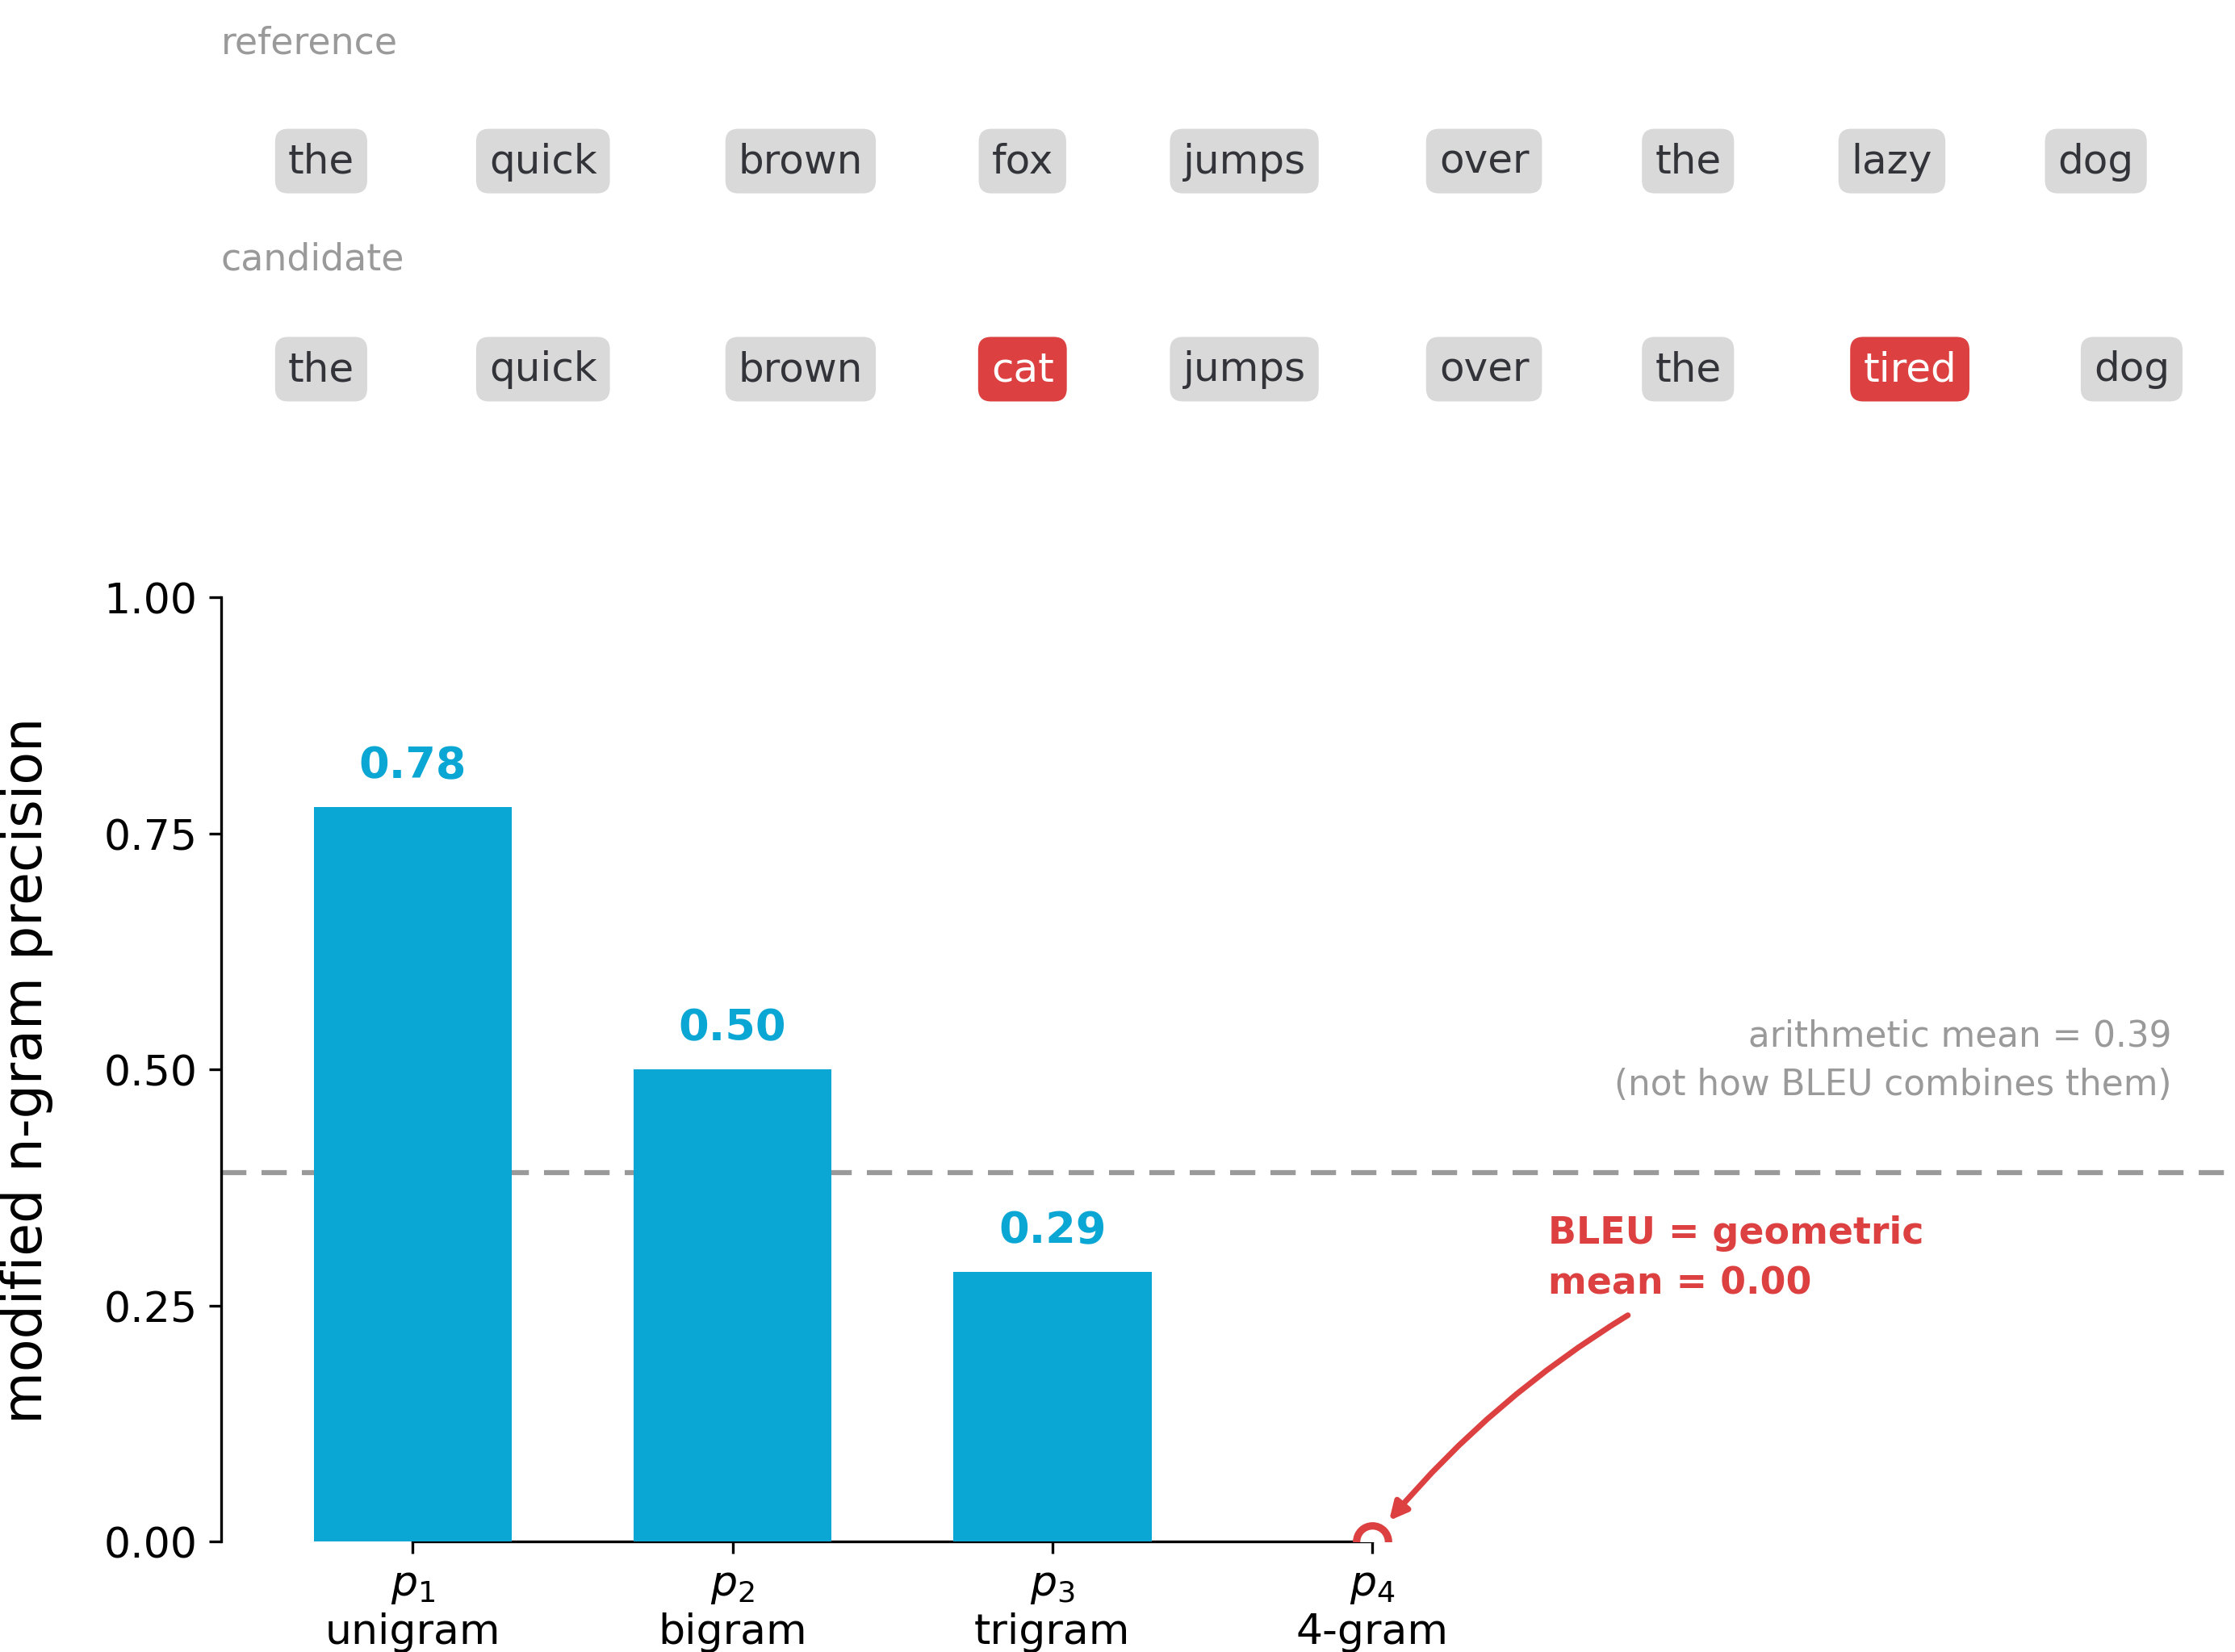
\includegraphics[width=0.62\textwidth]{figures/BLEU_ngram_precision.png}
\end{center}

\textbf{Figure. BLEU.} The candidate swaps two words, breaking every 4-gram, so the 4-gram precision $p_4$ is
$0$. Because BLEU is the geometric mean of the four precisions, that single zero drags the whole score
to $0$ --- even though $78\%$ of unigrams still match. An arithmetic mean would have reported $0.39$.
This is why sentence-level BLEU needs smoothing and is meant to be aggregated over a corpus.

\orangebox{Did you know that...}
{BLEU multiplies its n-gram precisions rather than averaging them: $\exp(\sum_n w_n \log p_n)$ is a
weighted \textbf{geometric} mean. The consequence is unforgiving --- if even one n-gram order has zero
matches, $\log 0 = -\infty$ and the whole score collapses to $0$, however good the lower orders are.
Introduced by Papineni et al. (2002) at IBM, BLEU was the first automatic MT metric to track human
judgment well enough to replace per-change human evaluation.}

\textbf{Other related metrics}

If BLEU is low but the translation reads correctly, the model is probably paraphrasing --- check METEOR
(credits synonyms and stems) or BERTScore (embedding similarity, see the GenAI chapter). TER reports the
same quality as an edit count rather than an overlap, and disagrees with BLEU on reordering, which it
penalizes more gently.

% ---------- Metric for Evaluation of Translation with Explicit ORdering ----------
% references:
% https://aclanthology.org/W05-0909.pdf

\clearpage
\thispagestyle{nlpstyle}
\section{METEOR}
\subsection{Metric for Evaluation of Translation with Explicit ORdering}

METEOR scores a translation the way a lenient grader would: it aligns the candidate to the reference
word by word, accepting not only exact matches but also stems (\textit{run}/\textit{running}) and
synonyms (\textit{quick}/\textit{fast}), then rewards how much of the reference it recovers. It exists
to fix the failure that hurts BLEU most --- a correct paraphrase worded differently. Where BLEU sees no
overlap and scores $0$, METEOR still credits the matched meaning.

% equation
\begin{center}
    \tikz{
        \node[inner sep=2pt, font=\Large] (a) {
            {
                $\displaystyle
                METEOR = (1 - {\color{nmlred}\gamma} \cdot {\color{nmlpurple}frag}^{\beta}) \cdot {\color{nmlcyan}F_{mean}}
                $
            }
        };
        \draw[overlay,-latex,nmlcyan, semithick] ($(a.north)+(2.5,-0.2)$) to[bend left=15] node[pos=1, right] {harmonic mean} +(1,.5);
        \draw[overlay,-latex,nmlpurple, semithick] ($(a.south)+(0.5,0.3)$) to[bend left=15] node[pos=1, left] {fragmentation penalty} +(-1,-.5);
    }
\end{center}

METEOR is the harmonic mean of unigram precision and recall (${\color{nmlcyan}F_{mean}}$), scaled down
by a fragmentation penalty (${\color{nmlred}\gamma}\cdot{\color{nmlpurple}frag}^{\beta}$) that grows as
matched words scatter out of order. It ranges from $0$ to $1$ and weights recall about nine times more
than precision, so recovering content matters more than staying terse.

\textbf{When to use METEOR?}

Use METEOR for translation and captioning when adequacy matters as much as exact wording, and for
morphologically rich or low-resource languages where exact n-gram matches are too strict. Avoid it when
you need cross-paper comparability (BLEU/sacreBLEU is standard) or when no stemmer or synonym resource
exists for your language --- the very thing that gives METEOR its edge.

\enlargethispage{\baselineskip}
\coloredboxes{
\item Credits synonyms and stems, so a fluent paraphrase scores near a literal translation --- exactly
where BLEU collapses to $0$ (see figure).
\item Correlates with human judgment at the \textit{sentence} level, not just the corpus level, because
precision, recall, and word order fold into one stable, recall-weighted score.
}
{
\item Needs linguistic resources. Stemmers and synonym tables (e.g.\ WordNet) must exist for the target
language; quality drops where they don't.
\item Slower and less standardized than BLEU. The alignment step and tunable parameters
($\alpha,\gamma,\beta$) mean two papers' METEOR numbers may not be comparable.
}

\clearpage

\thispagestyle{customstyle}

\begin{center}
    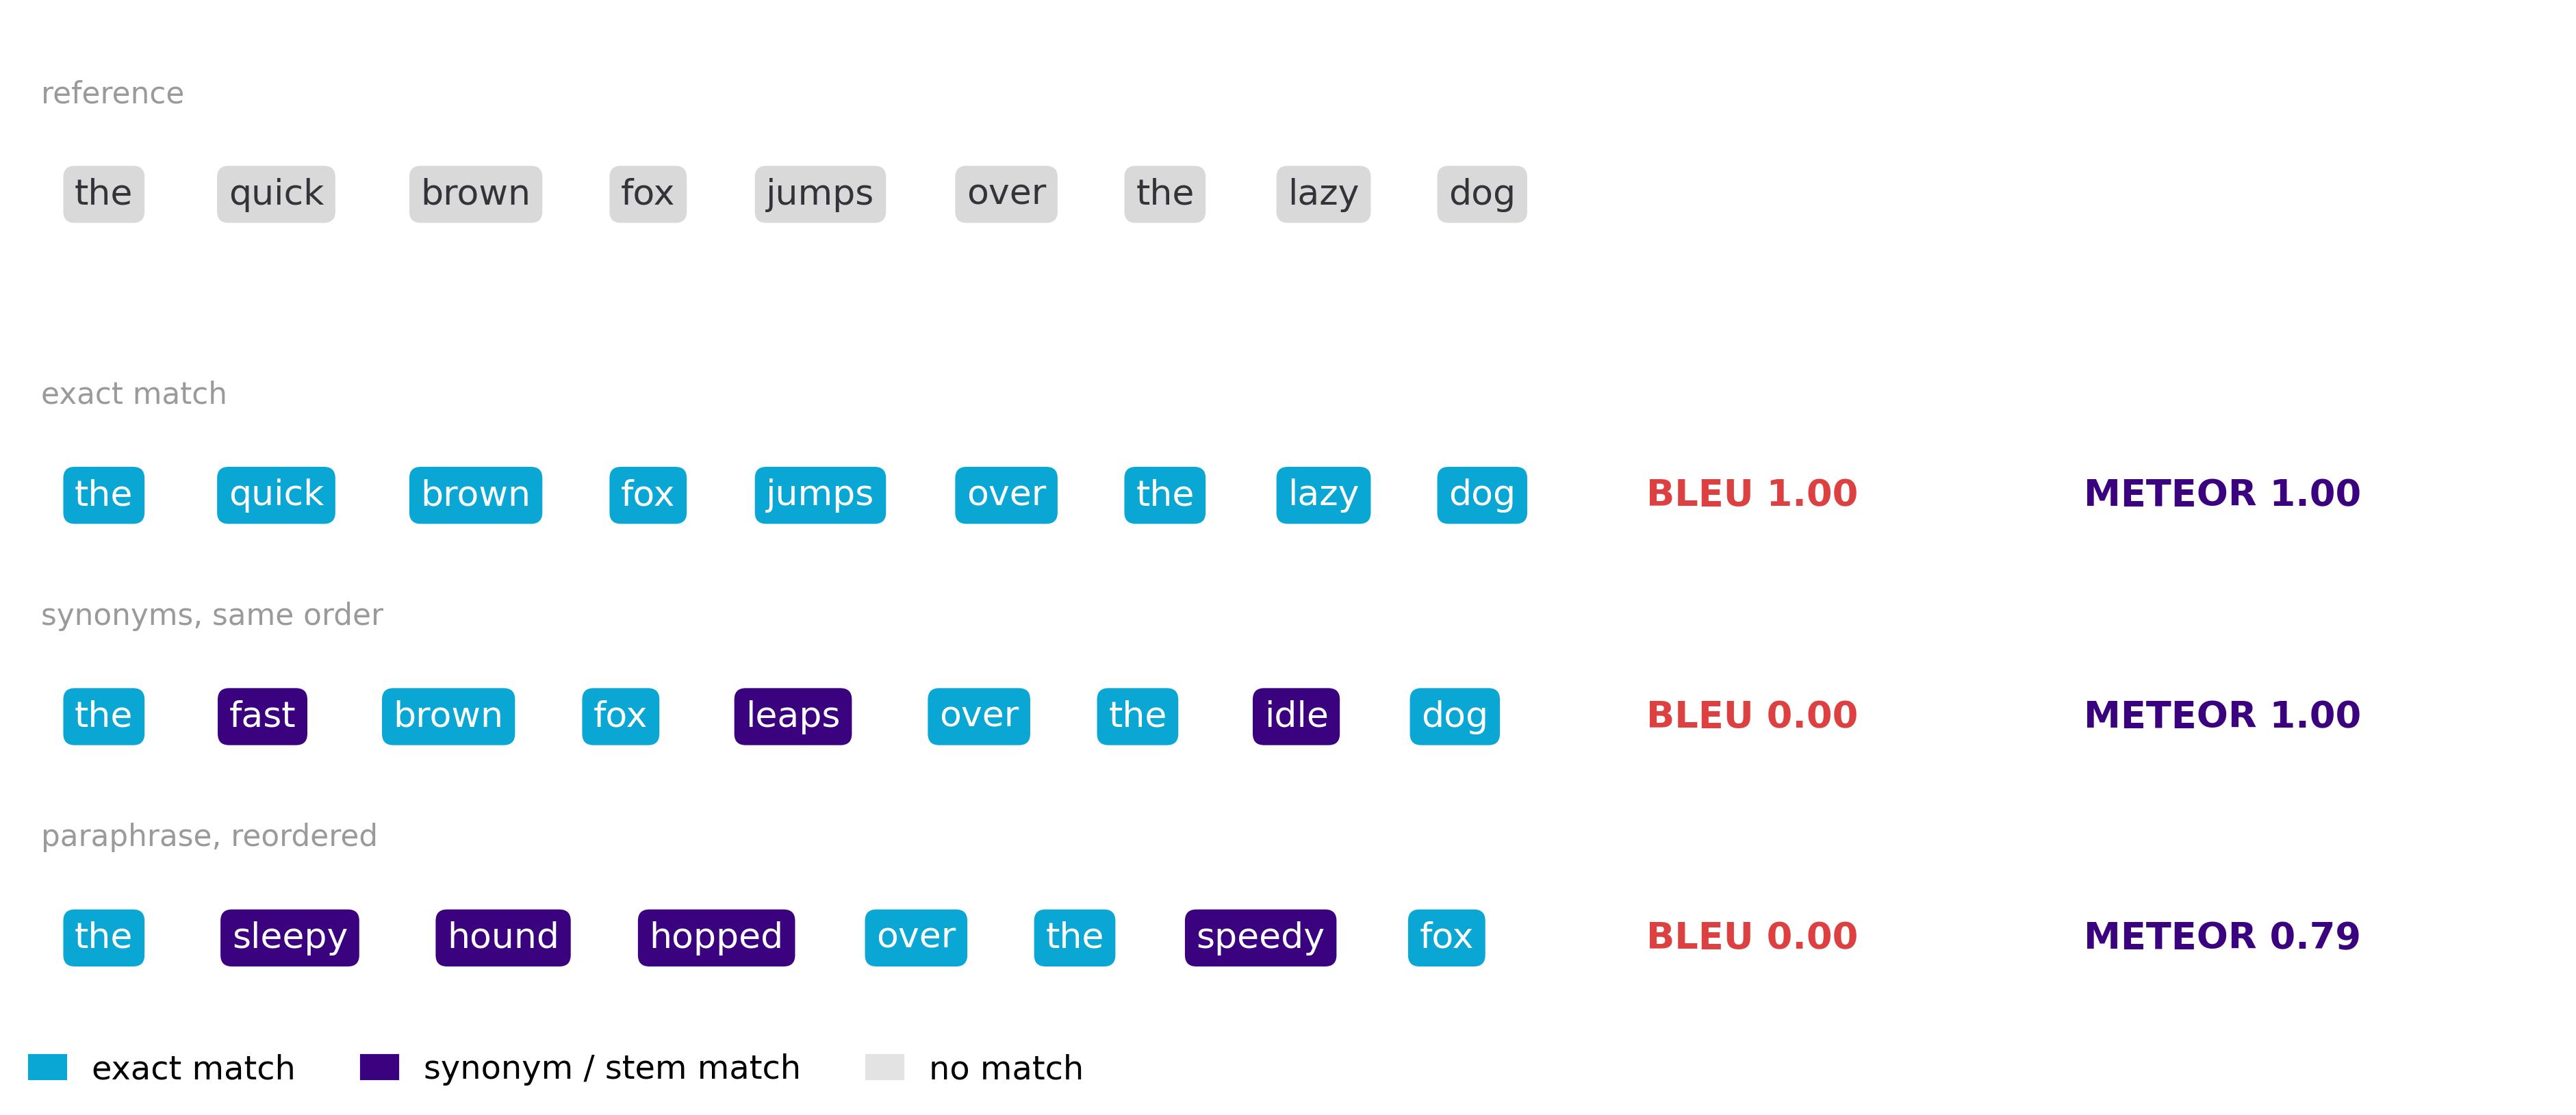
\includegraphics[width=\textwidth]{figures/METEOR_vs_BLEU.png}
\end{center}

\textbf{Figure. METEOR.} One reference scored against three candidates. Replacing words with synonyms
(\textit{fast}, \textit{leaps}, \textit{idle}) breaks every n-gram, so BLEU falls to $0$, but METEOR
matches them through its synonym and stem tables and stays at $1.0$. Reordering the paraphrase keeps the
matched words but scatters them, so METEOR's fragmentation penalty docks it to $0.79$ while BLEU again
reads $0$.

\orangebox{Did you know that...}
{METEOR's harmonic mean is deliberately unbalanced: $F_{mean} = \frac{P\cdot R}{\alpha P + (1-\alpha)R}$
with $\alpha = 0.9$, so recall carries nine times the weight of precision. A translation that recovers
all of the reference's meaning but adds a few words is barely penalized; one that drops content is hit
hard --- adequacy over brevity, by design. Developed at Carnegie Mellon (Banerjee \& Lavie, 2005) as a
direct response to BLEU.}

\textbf{Other related metrics}

A large METEOR--BLEU gap means the model is conveying the meaning with different words, not making
errors --- the paraphrase case BLEU cannot see. For a surface edit-based view compare TER; for
embedding-based similarity that needs no synonym table, see BERTScore in the GenAI chapter.

% ---------- Recall-Oriented Understudy for Gisting Evaluation ----------
% references:
% https://aclanthology.org/W04-1013.pdf
% https://aclanthology.org/E17-2007.pdf

\clearpage
\thispagestyle{nlpstyle}
\section{ROUGE}
\subsection{Recall-Oriented Understudy for Gisting Evaluation}

ROUGE evaluates a summary by how much of the reference it recovers: it counts overlapping unigrams
(ROUGE-1), bigrams (ROUGE-2), or the longest common subsequence (ROUGE-L), divided by the reference
total. It reports recall rather than precision because in summarization the risk is leaving content out,
not adding a little extra.

% equation
\begin{center}
    \tikz{
        \node[inner sep=2pt, font=\Large] (a) {
            {
                $\displaystyle
                ROUGE\text{-}N = \frac{\sum_{s \in Ref} \sum_{gram_n \in s} {\color{nmlcyan}Count_{match}}(gram_n)}{\sum_{s \in Ref} \sum_{gram_n \in s} {\color{nmlpurple}Count}(gram_n)}
                $
            }
        };
        \draw[overlay,-latex,nmlcyan, semithick] ($(a.north)+(2.0,-0.1)$) to[bend left=15] node[pos=1, right] {matching n-grams} +(1,.5);
        \draw[overlay,-latex,nmlpurple, semithick] ($(a.south)+(2.0,0.3)$) to[bend left=15] node[pos=1, left] {total reference n-grams} +(-1,-.5);
    }
\end{center}

ROUGE ranges from $0$ to $1$; the variant matters more than the absolute number. ROUGE-1 captures content
overlap, ROUGE-2 local fluency (word pairs), and ROUGE-L in-order overlap. Report ROUGE-1 and ROUGE-L
together --- a high ROUGE-1 with a low ROUGE-L means the right words in the wrong order.

\textbf{When to use ROUGE?}

Use ROUGE for summarization and tasks scored against reference text where coverage is the priority
(headline generation, extractive QA). Avoid recall-only ROUGE when verbosity matters --- a padded summary
keeps full recall while precision collapses (see figure); report ROUGE-F or a length budget instead. For
meaning over wording, use BERTScore.

\enlargethispage{\baselineskip}
\coloredboxes{
\item Cheap and reproducible: pure n-gram counting, scaling to thousands of summaries with no model to run.
\item The variant set is diagnostic --- ROUGE-1 vs ROUGE-2 vs ROUGE-L localizes a gap to content, local
fluency, or ordering.
}
{
\item Recall-only by default rewards length: a summary that copies the whole document earns near-perfect
recall, and only precision (usually unreported) catches the padding (see figure).
\item Lexical, not semantic. A correct abstractive paraphrase scores low; even human-written summaries
can score poorly under ROUGE.
}

\clearpage

\thispagestyle{customstyle}

\begin{center}
    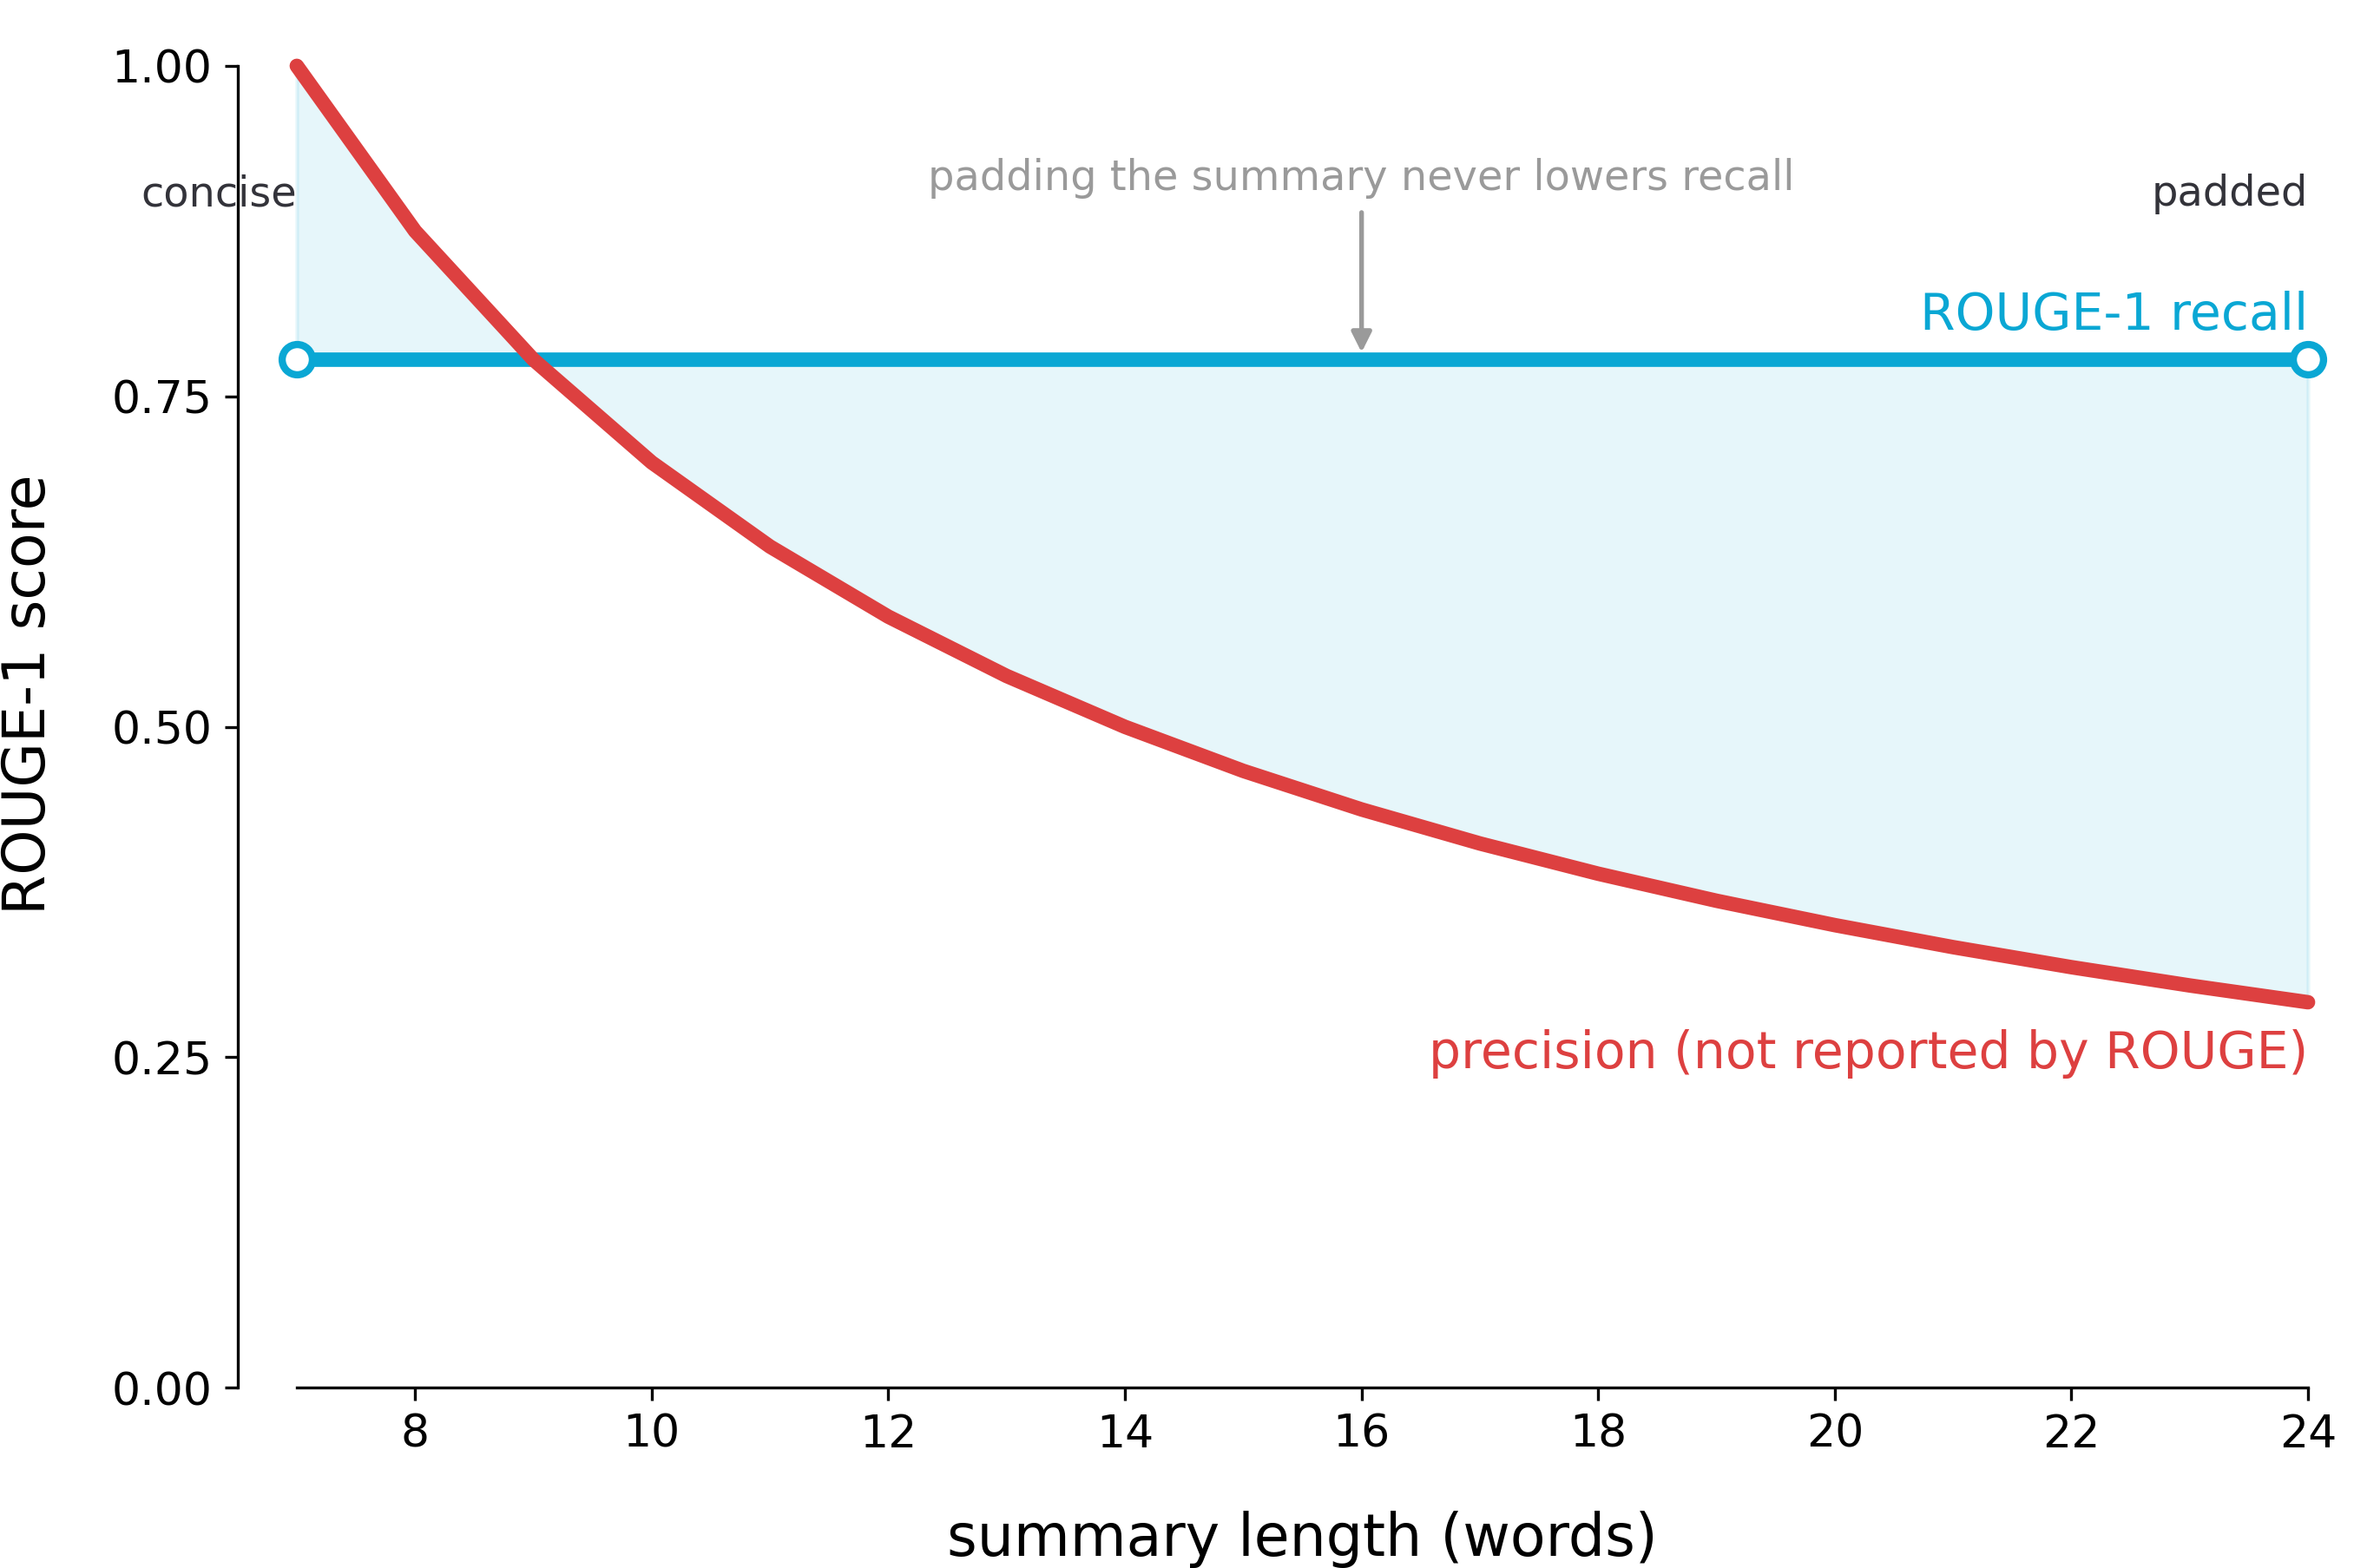
\includegraphics[width=0.6\textwidth]{figures/ROUGE_variants.png}
\end{center}

\textbf{Figure. ROUGE.} A concise summary already covers the reference, so its ROUGE-1 recall is $0.78$.
Appending filler words that aren't in the reference cannot lower recall --- it stays flat at $0.78$ ---
while precision falls from $1.0$ to $0.29$. Recall, the number ROUGE reports, is blind to padding; only
precision, which it omits, sees it.

\orangebox{Did you know that...}
{Because plain ROUGE is recall, it can only rise or stay flat as a summary grows: extra words never
remove a reference match, they only add chances for new ones. A system that emits the entire source
document scores near-perfect ROUGE recall while being useless as a summary --- which is why leaderboards
pair ROUGE with a length limit or report the F-score. Introduced by Chin-Yew Lin (2004); the name stands
for Recall-Oriented Understudy for Gisting Evaluation.}

\textbf{Other related metrics}

ROUGE is the recall-shaped mirror of BLEU's precision: to penalize over-generation, BLEU or ROUGE-F is
the better lens. A high ROUGE-1 with a low ROUGE-2 or ROUGE-L flags right-content, wrong-order. For
credit beyond exact tokens, see BERTScore in the GenAI chapter.

% ---------- Translation Error Rate ----------
% reference: https://aclanthology.org/2006.amta-papers.25.pdf
\clearpage
\thispagestyle{nlpstyle}
\section{TER}
\subsection{Translation Error Rate}

TER reports translation quality as post-editing effort: the fraction of edits a human would need to turn
the machine output into the reference. It counts insertions, deletions, substitutions, and --- unlike
word-error metrics --- shifts, where a whole phrase moves to a new position. A TER of $0.2$ means roughly
one edit per five reference words; lower is better.

% equation
\begin{center}
    \tikz{
        \node[inner sep=2pt, font=\Large] (a) {
            {
                $\displaystyle
                TER = \frac{{\color{nmlcyan}\text{insertions}} + {\color{nmlcyan}\text{deletions}} + {\color{nmlcyan}\text{substitutions}} + {\color{nmlpurple}\text{shifts}}}{{\color{nmlred}\text{reference length}}}
                $
            }
        };
        \draw[overlay,-latex,nmlcyan, semithick] ($(a.north)+(0.0,-0.1)$) to[bend right=15] node[pos=1, left] {word-level edits} +(-1,.5);
        \draw[overlay,-latex,nmlpurple, semithick] ($(a.north)+(2.7,-0.1)$) to[bend left=15] node[pos=1, right] {sequence shifts} +(0.0,.5);
        \draw[overlay,-latex,nmlred, semithick] ($(a.south)+(2.0,0.3)$) to[bend left=15] node[pos=1, left] {words in reference} +(-1,-.5);
    }
\end{center}

TER starts at $0$ (no edits) and can exceed $1$ when the output needs more edits than the reference has
words. Because it counts edits over reference length, TER reads directly as edits per reference word ---
which is why it tracks human post-editing time more closely than overlap scores.

\textbf{When to use TER?}

Use TER when the downstream cost is human post-editing: translation-memory pipelines, localization
vendors paid per edit. Its shift operation suits frequent reordering --- one moved phrase, one edit.
Avoid TER when correct paraphrases use different words (every substitution is an error; use METEOR or
BERTScore), and for leaderboards, where BLEU is the convention.

\enlargethispage{\baselineskip}
\coloredboxes{
\item Interpretable as work. A TER of $0.3$ estimates three edits per ten words --- a number a
localization manager can convert into hours and cost.
\item Handles reordering. The shift moves a whole phrase for one edit, so a correctly translated but
relocated clause isn't punished as several substitutions (see figure).
}
{
\item Surface-level. Different-but-correct word choices count as substitutions; TER has no notion of
synonymy.
\item Tends to overestimate effort. Its shift search is a greedy heuristic, not optimal, so it can
report more edits than a human would actually make.
}

\clearpage

\thispagestyle{customstyle}

\begin{center}
    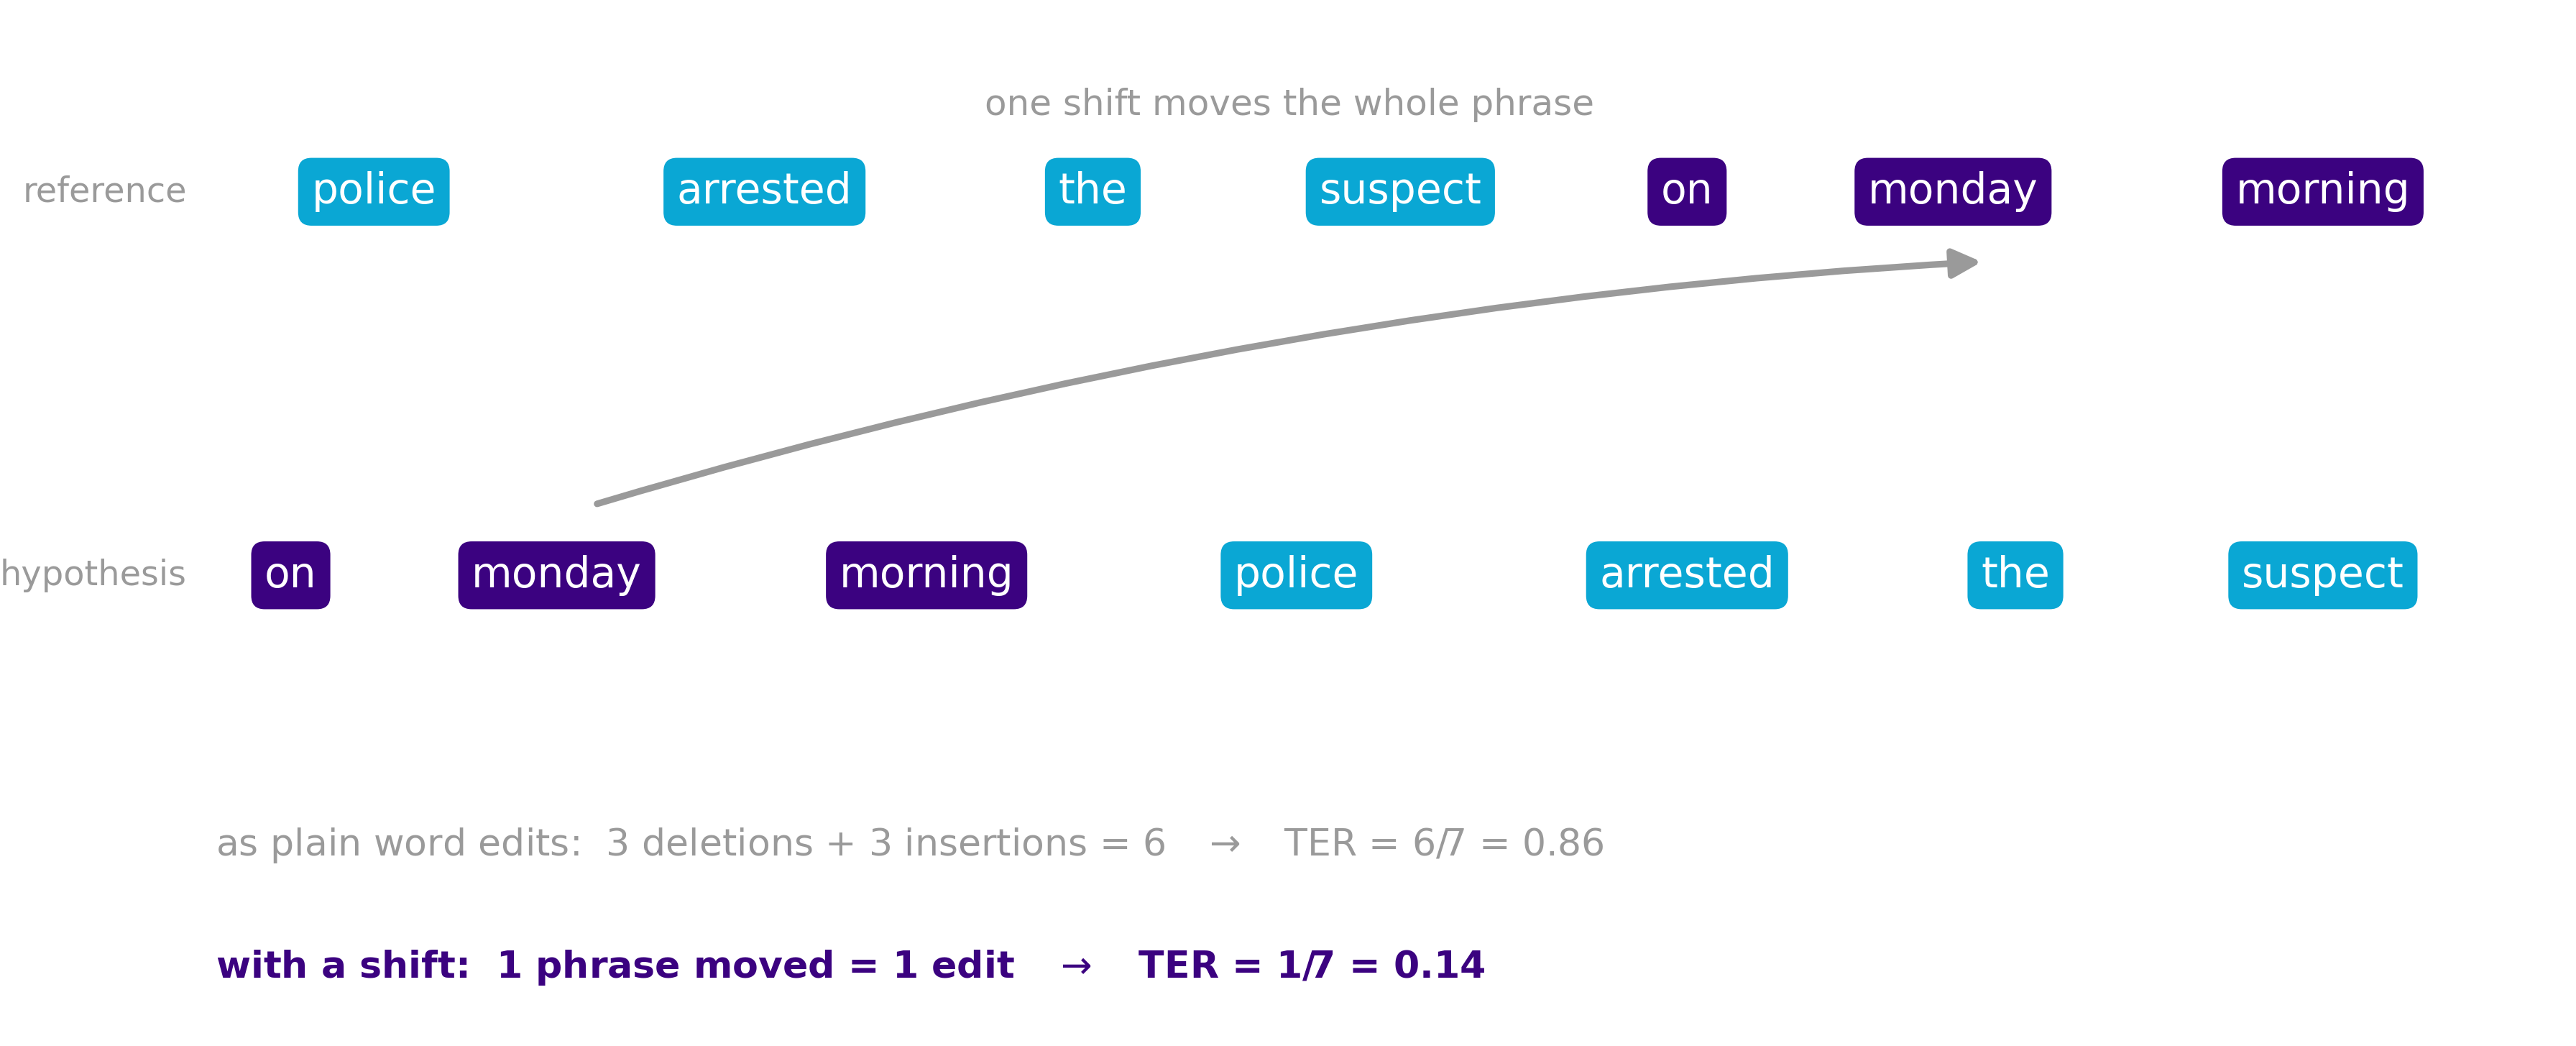
\includegraphics[width=\textwidth]{figures/TER_edit_breakdown.png}
\end{center}

\textbf{Figure. TER.} The hypothesis is the reference with the phrase \textit{on monday morning} moved to the
front. Scored as plain word edits, relocating the three-word phrase costs three deletions plus three
insertions ($\text{TER}=6/7=0.86$). TER's shift operation moves the whole phrase as a single edit
($\text{TER}=1/7=0.14$), matching the one drag a human editor would actually perform.

\orangebox{Did you know that...}
{The shift is what separates TER from word error rate. WER must delete every word of a misplaced phrase
and re-insert it elsewhere --- six edits for a three-word move --- so it punishes reordering harshly.
TER charges one edit for the move, whatever the phrase length or distance, because that mirrors the
single action a human takes. Finding the optimal set of shifts is expensive, so TER uses a greedy
approximation. Introduced by Snover et al.\ (2006).}

\textbf{Other related metrics}

TER and WER are the same edit-distance idea; TER adds the shift, so on reordered output TER is far lower
than a WER-style count. Against BLEU it often ranks systems differently, forgiving the reordering that
BLEU's n-grams punish. Lower TER is better --- the opposite direction to BLEU and METEOR.

% ---------- Exact Match ----------
% reference: https://nlp.stanford.edu/pubs/rajpurkar2016squad.pdf
\clearpage
\thispagestyle{nlpstyle}
\section{EM}
\subsection{Exact Match}

Exact Match is the fraction of predictions identical to the reference: each scores $1$ if it matches the
gold answer exactly --- after light normalization (lowercasing, stripping punctuation and articles) ---
and $0$ otherwise. It is the strictest text metric: \textit{Martin Luther King Jr.} scores $0$ against
the gold \textit{Martin Luther King}, the same score as a completely wrong answer (see figure).

% equation
\begin{center}
    \tikz{
        \node[inner sep=2pt, font=\Large] (a) {
            {
                $\displaystyle
                EM = \frac{1}{{\color{nmlred}N}} \sum_{i=1}^{N} {\color{nmlgreen}\mathds{1}}({\color{nmlpurple}\hat{y}_i} = {\color{nmlcyan}y_i})
                $
            }
        };
        \draw[overlay,-latex,nmlred, semithick] ($(a.south)+(-0.5,0.2)$) to[bend left=15] node[pos=1, left] {number of samples} +(-1,-.5);
        \draw[overlay,-latex,nmlpurple, semithick] ($(a.north)+(1.0,-0.2)$) to[bend right=15] node[pos=1, left] {predicted text} +(-1,.5);
        \draw[overlay,-latex,nmlcyan, semithick] ($(a.north)+(1.9,-0.2)$) to[bend left=15] node[pos=1, right] {reference text} +(1,.5);
    }
\end{center}

EM ranges from $0$ to $1$. Being all-or-nothing per example, it is most informative when the answer is
short and canonical; on long outputs it sits near $0$ even for good predictions, so it is usually paired
with token-level F1, which scores partial word overlap.

\textbf{When to use EM?}

Use EM where only an exact answer is acceptable: extractive QA spans, structured outputs (JSON keys, SQL,
API arguments), classification cast as text. Avoid it for open-ended or long-form generation, where it
bottoms out near $0$ even for strong outputs --- use token-F1, ROUGE, or BERTScore for graded credit.

\enlargethispage{\baselineskip}
\coloredboxes{
\item Unambiguous and trivial to explain: the prediction is either right or wrong, with no threshold to
tune.
\item Strict correctness guarantee. When any deviation breaks downstream use --- a malformed JSON key, a
wrong SQL clause --- EM is exactly the bar that matters.
}
{
\item All-or-nothing. A prediction off by one token scores $0$, identical to a fully wrong one:
\textit{Martin Luther King Jr.} and \textit{Malcolm X} both score $0$ against the gold (see figure).
\item Normalization-sensitive. Whether casing, punctuation, and articles are stripped before comparison
can swing EM by several points, so the scheme must be reported.
}

\clearpage

\begin{center}
    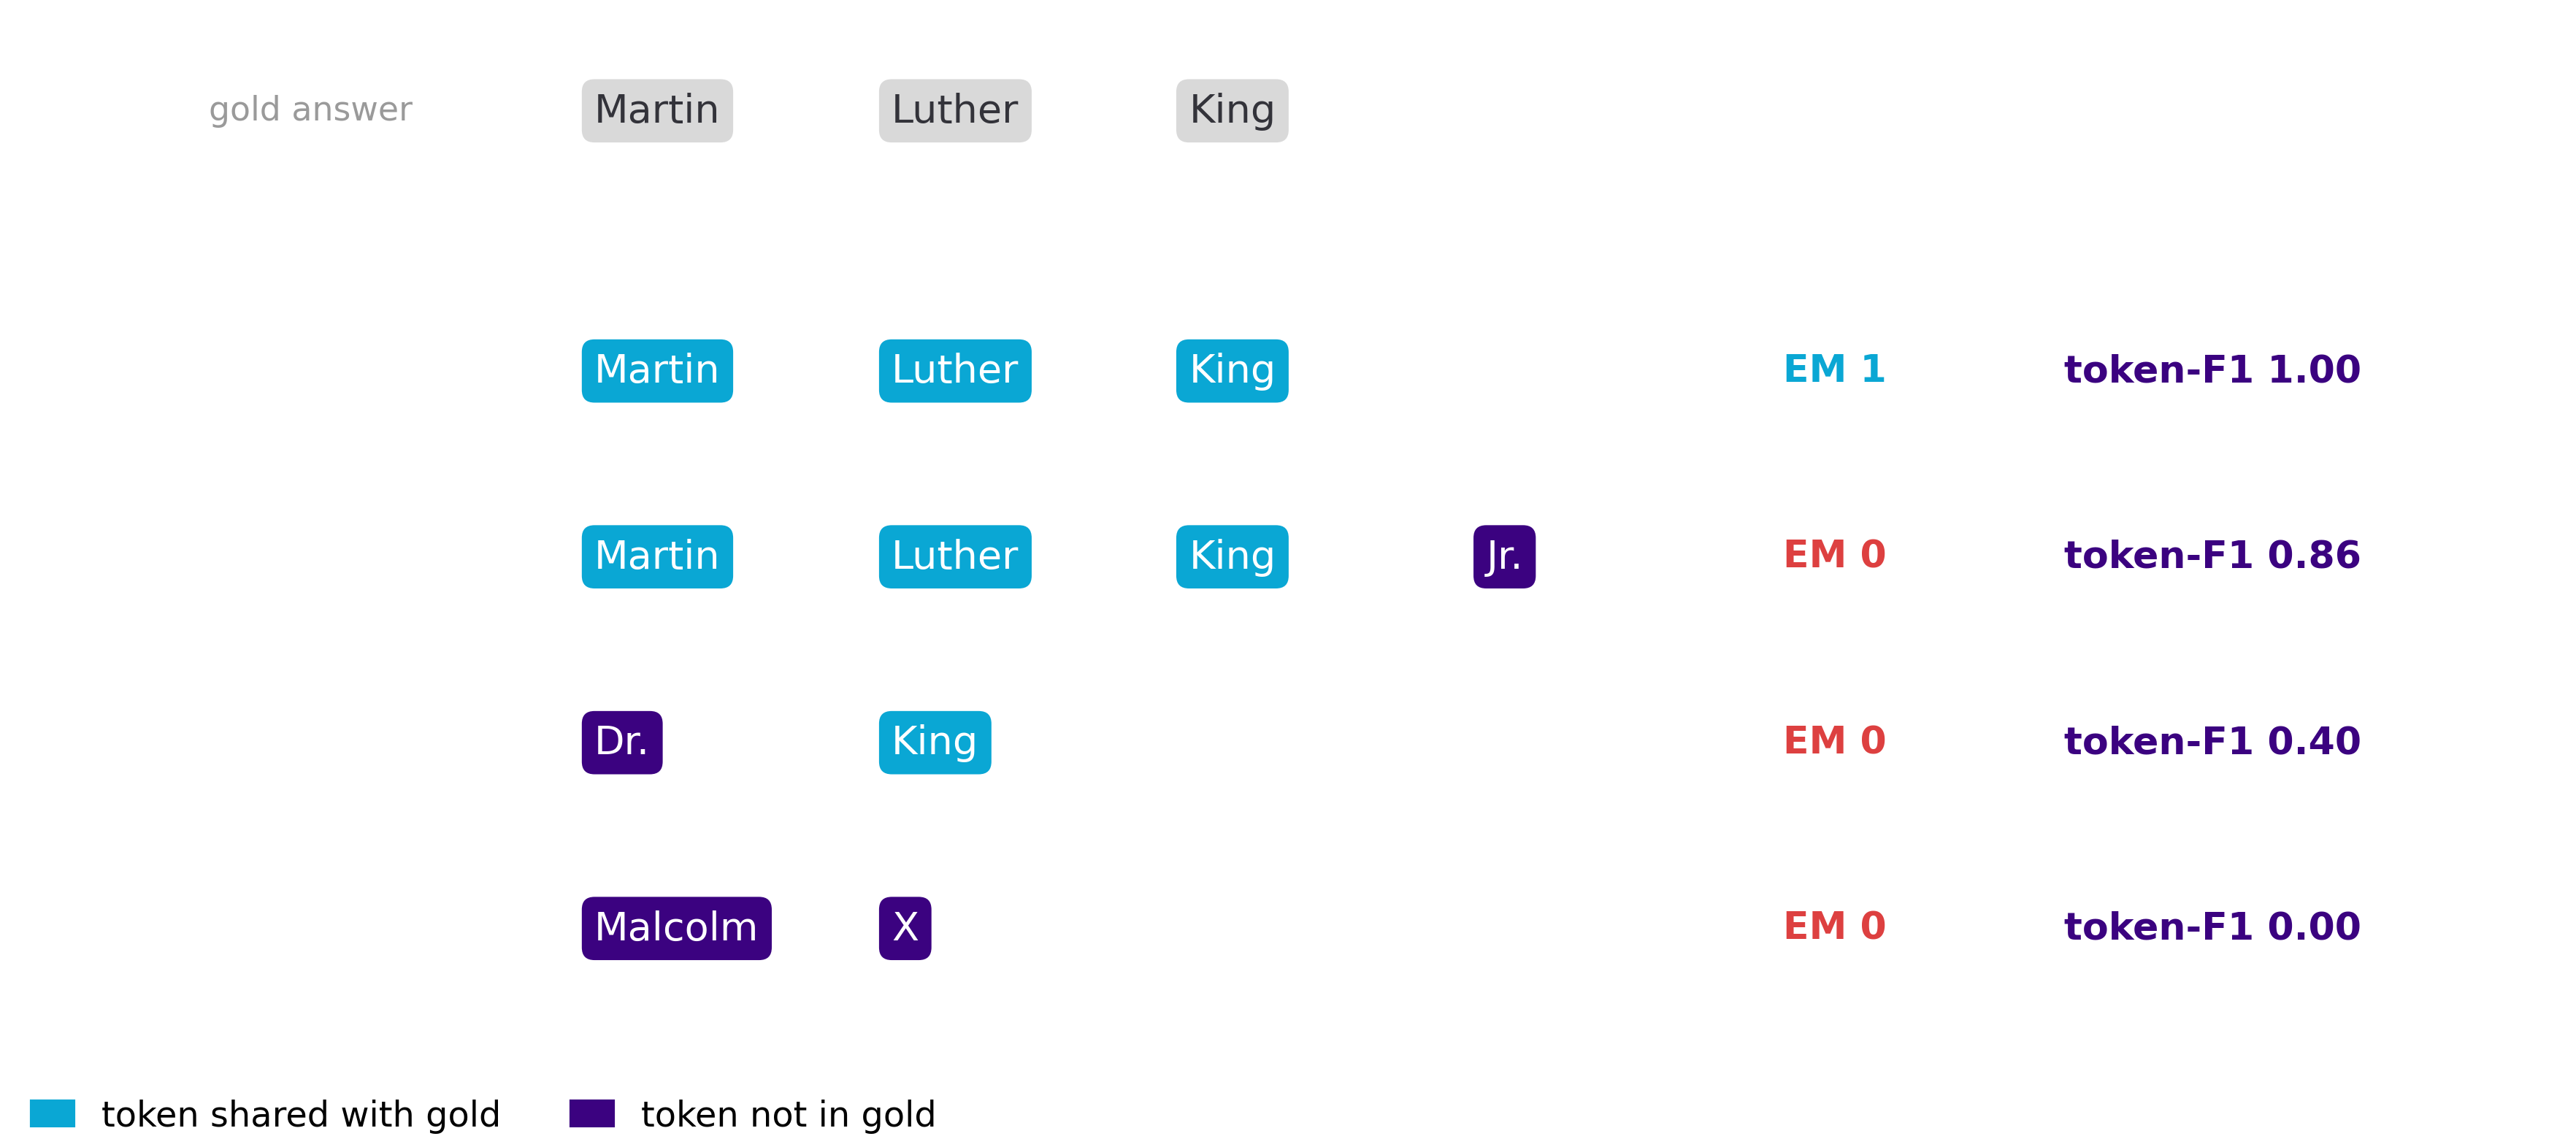
\includegraphics[width=0.95\textwidth]{figures/EM_vs_F1.png}
\end{center}

\textbf{Figure. EM.} Four predictions against the gold answer \textit{Martin Luther King}. Only the exact
match scores EM $=1$; adding \textit{Jr.}, abbreviating to \textit{Dr.\ King}, or answering
\textit{Malcolm X} all score EM $=0$. Token-level F1 instead grades the overlap --- $0.86$, $0.40$,
$0.00$ --- giving the partial credit EM withholds.

\orangebox{Did you know that...}
{Exact Match anchors the Stanford Question Answering Dataset (SQuAD) benchmark, always paired with
token-level F1. Token-F1 treats each answer as a bag of words and takes the harmonic mean of how many
predicted tokens appear in the gold answer (precision) and how many gold tokens were recovered (recall)
--- so \textit{Martin Luther King Jr.} earns F1 $=0.86$ for its three correct tokens while EM gives it
nothing. EM reports exact correctness; F1 reports how close the near-misses came.}

\textbf{Other related metrics}

EM and token-F1 are read together: a large F1--EM gap means the model is almost right --- correct
content, wrong boundaries or extra words --- rather than wrong. For n-gram overlap on longer text, see
BLEU or ROUGE; for semantic equivalence, BERTScore.

% ---------- Word Error Rate ----------
\clearpage
\thispagestyle{nlpstyle}
\section{WER}
\subsection{Word Error Rate}

WER scores a speech recognizer by how many word-level edits separate its transcript from the reference:
count the substitutions, deletions, and insertions in the best alignment, then divide by the number of
reference words. A WER of $0.1$ means one word in ten is wrong. It is the standard yardstick for ASR
because transcription errors are naturally counted in words.

% equation
\begin{center}
    \tikz{
        \node[inner sep=2pt, font=\Large] (a) {
            {
                $\displaystyle
                WER = \frac{{\color{nmlcyan}S} + {\color{nmlcyan}D} + {\color{nmlcyan}I}}{{\color{nmlred}N}}
                $
            }
        };
        \draw[overlay,-latex,nmlcyan, semithick] ($(a.north)+(0.5,-0.1)$) to[bend right=15] node[pos=1, left] {edit operations} +(-1,.5);
        \draw[overlay,-latex,nmlred, semithick] ($(a.south)+(1.0,0.2)$) to[bend left=15] node[pos=1, left] {words in reference} +(-1,-.5);
    }
\end{center}

WER starts at $0$ and can exceed $1$ ($100\%$) when a transcript inserts more wrong words than the
reference has. The three error types are diagnostic on their own: many insertions point to a decoder that
hallucinates words, many deletions to dropped speech, substitutions to confusable words (see figure).

\textbf{When to use WER?}

Use WER for ASR, voice assistants, and dictation, where every word should be transcribed correctly. Avoid
it when meaning survives the errors --- \textit{can't} versus \textit{cannot} is one substitution but no
change in meaning --- and for character-based or tonal languages, where Character Error Rate (CER), the
same formula per character, fits better.

\enlargethispage{\baselineskip}
\coloredboxes{
\item Diagnostic by construction. Splitting errors into substitutions, deletions, and insertions points
at the failure mode, not just its size (see figure).
\item Standard and interpretable. ``One word in ten wrong'' is understood across the field, making WER
comparable across systems and datasets.
}
{
\item Blind to meaning and importance. Every word counts equally: misrecognizing a critical digit and
dropping a filler ``um'' both cost one edit, though only one changes the message.
\item Sensitive to normalization. Punctuation, casing, contractions, and number formatting must be
standardized first, or formatting differences inflate WER with no real recognition error.
}

\clearpage

\begin{center}
    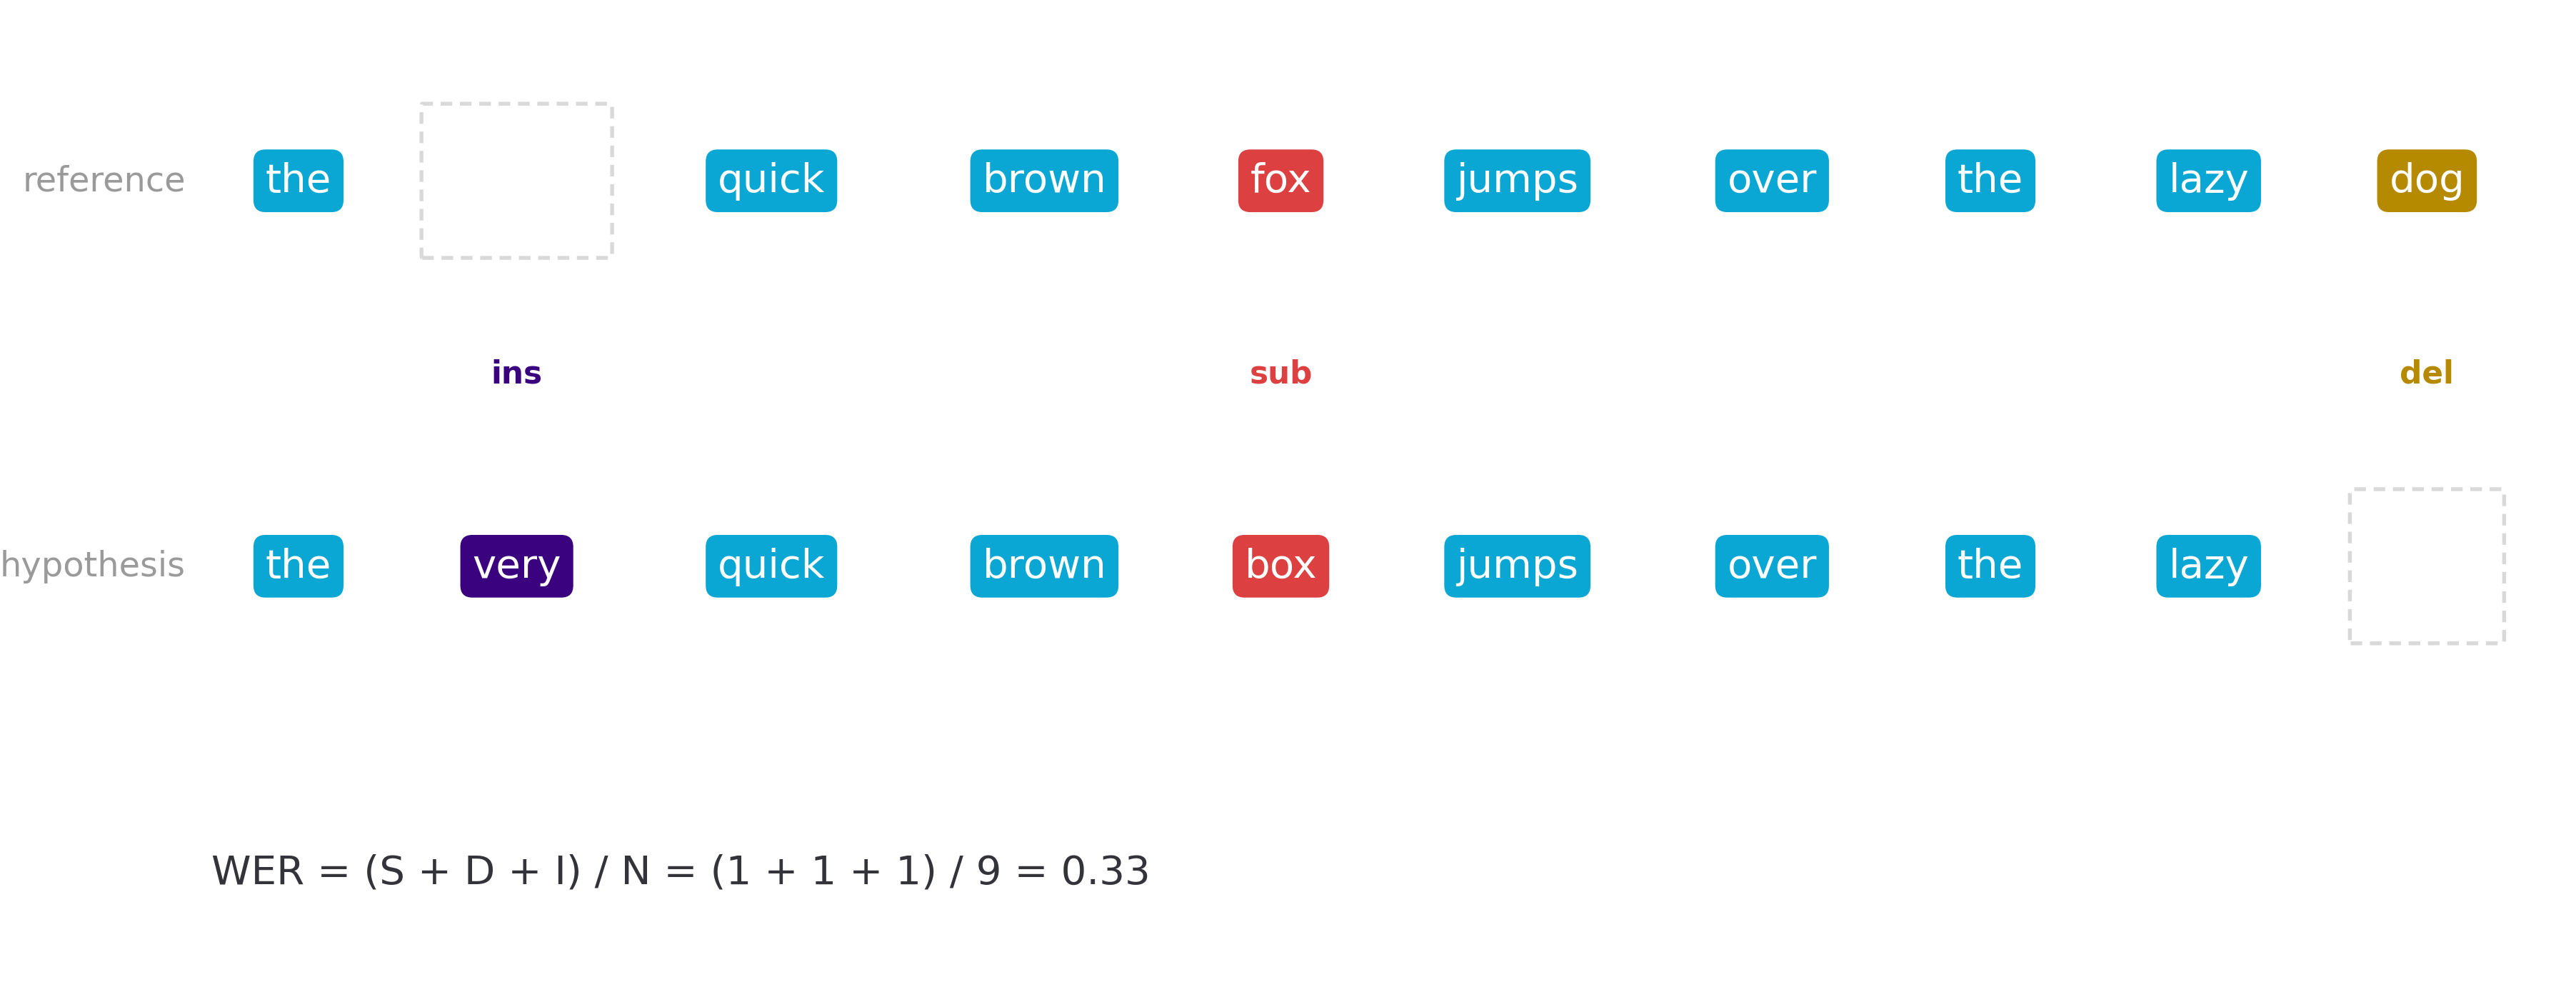
\includegraphics[width=\textwidth]{figures/WER_vs_errors.png}
\end{center}

\textbf{Figure. WER.} The best alignment between reference and hypothesis splits the errors into one
substitution (\textit{fox}\,$\rightarrow$\,\textit{box}), one deletion (\textit{dog}), and one insertion
(\textit{very}). WER sums them over the reference length: $(1+1+1)/9 = 0.33$. That same alignment is what
lets WER report \textit{which} kind of error dominates, not merely how many.

\orangebox{Did you know that...}
{WER is the Levenshtein (edit) distance computed over words instead of characters, normalized by the
reference length. The substitution, deletion, and insertion counts come from the \textit{minimum-cost}
alignment, found by dynamic programming --- so the split into error types is the cheapest explanation of
the differences, not the only one. Run the identical computation per character and you get Character
Error Rate (CER). The distance was introduced by Levenshtein in 1965.}

\textbf{Other related metrics}

WER and TER share the edit-distance core; TER adds a shift operation, so on reordered output (common in
translation, rare in transcription) TER reads far lower. For languages where word boundaries are unclear,
CER applies the identical formula per character. For meaning-level scoring beyond surface edits, see
BERTScore.